\begin{figure*}
    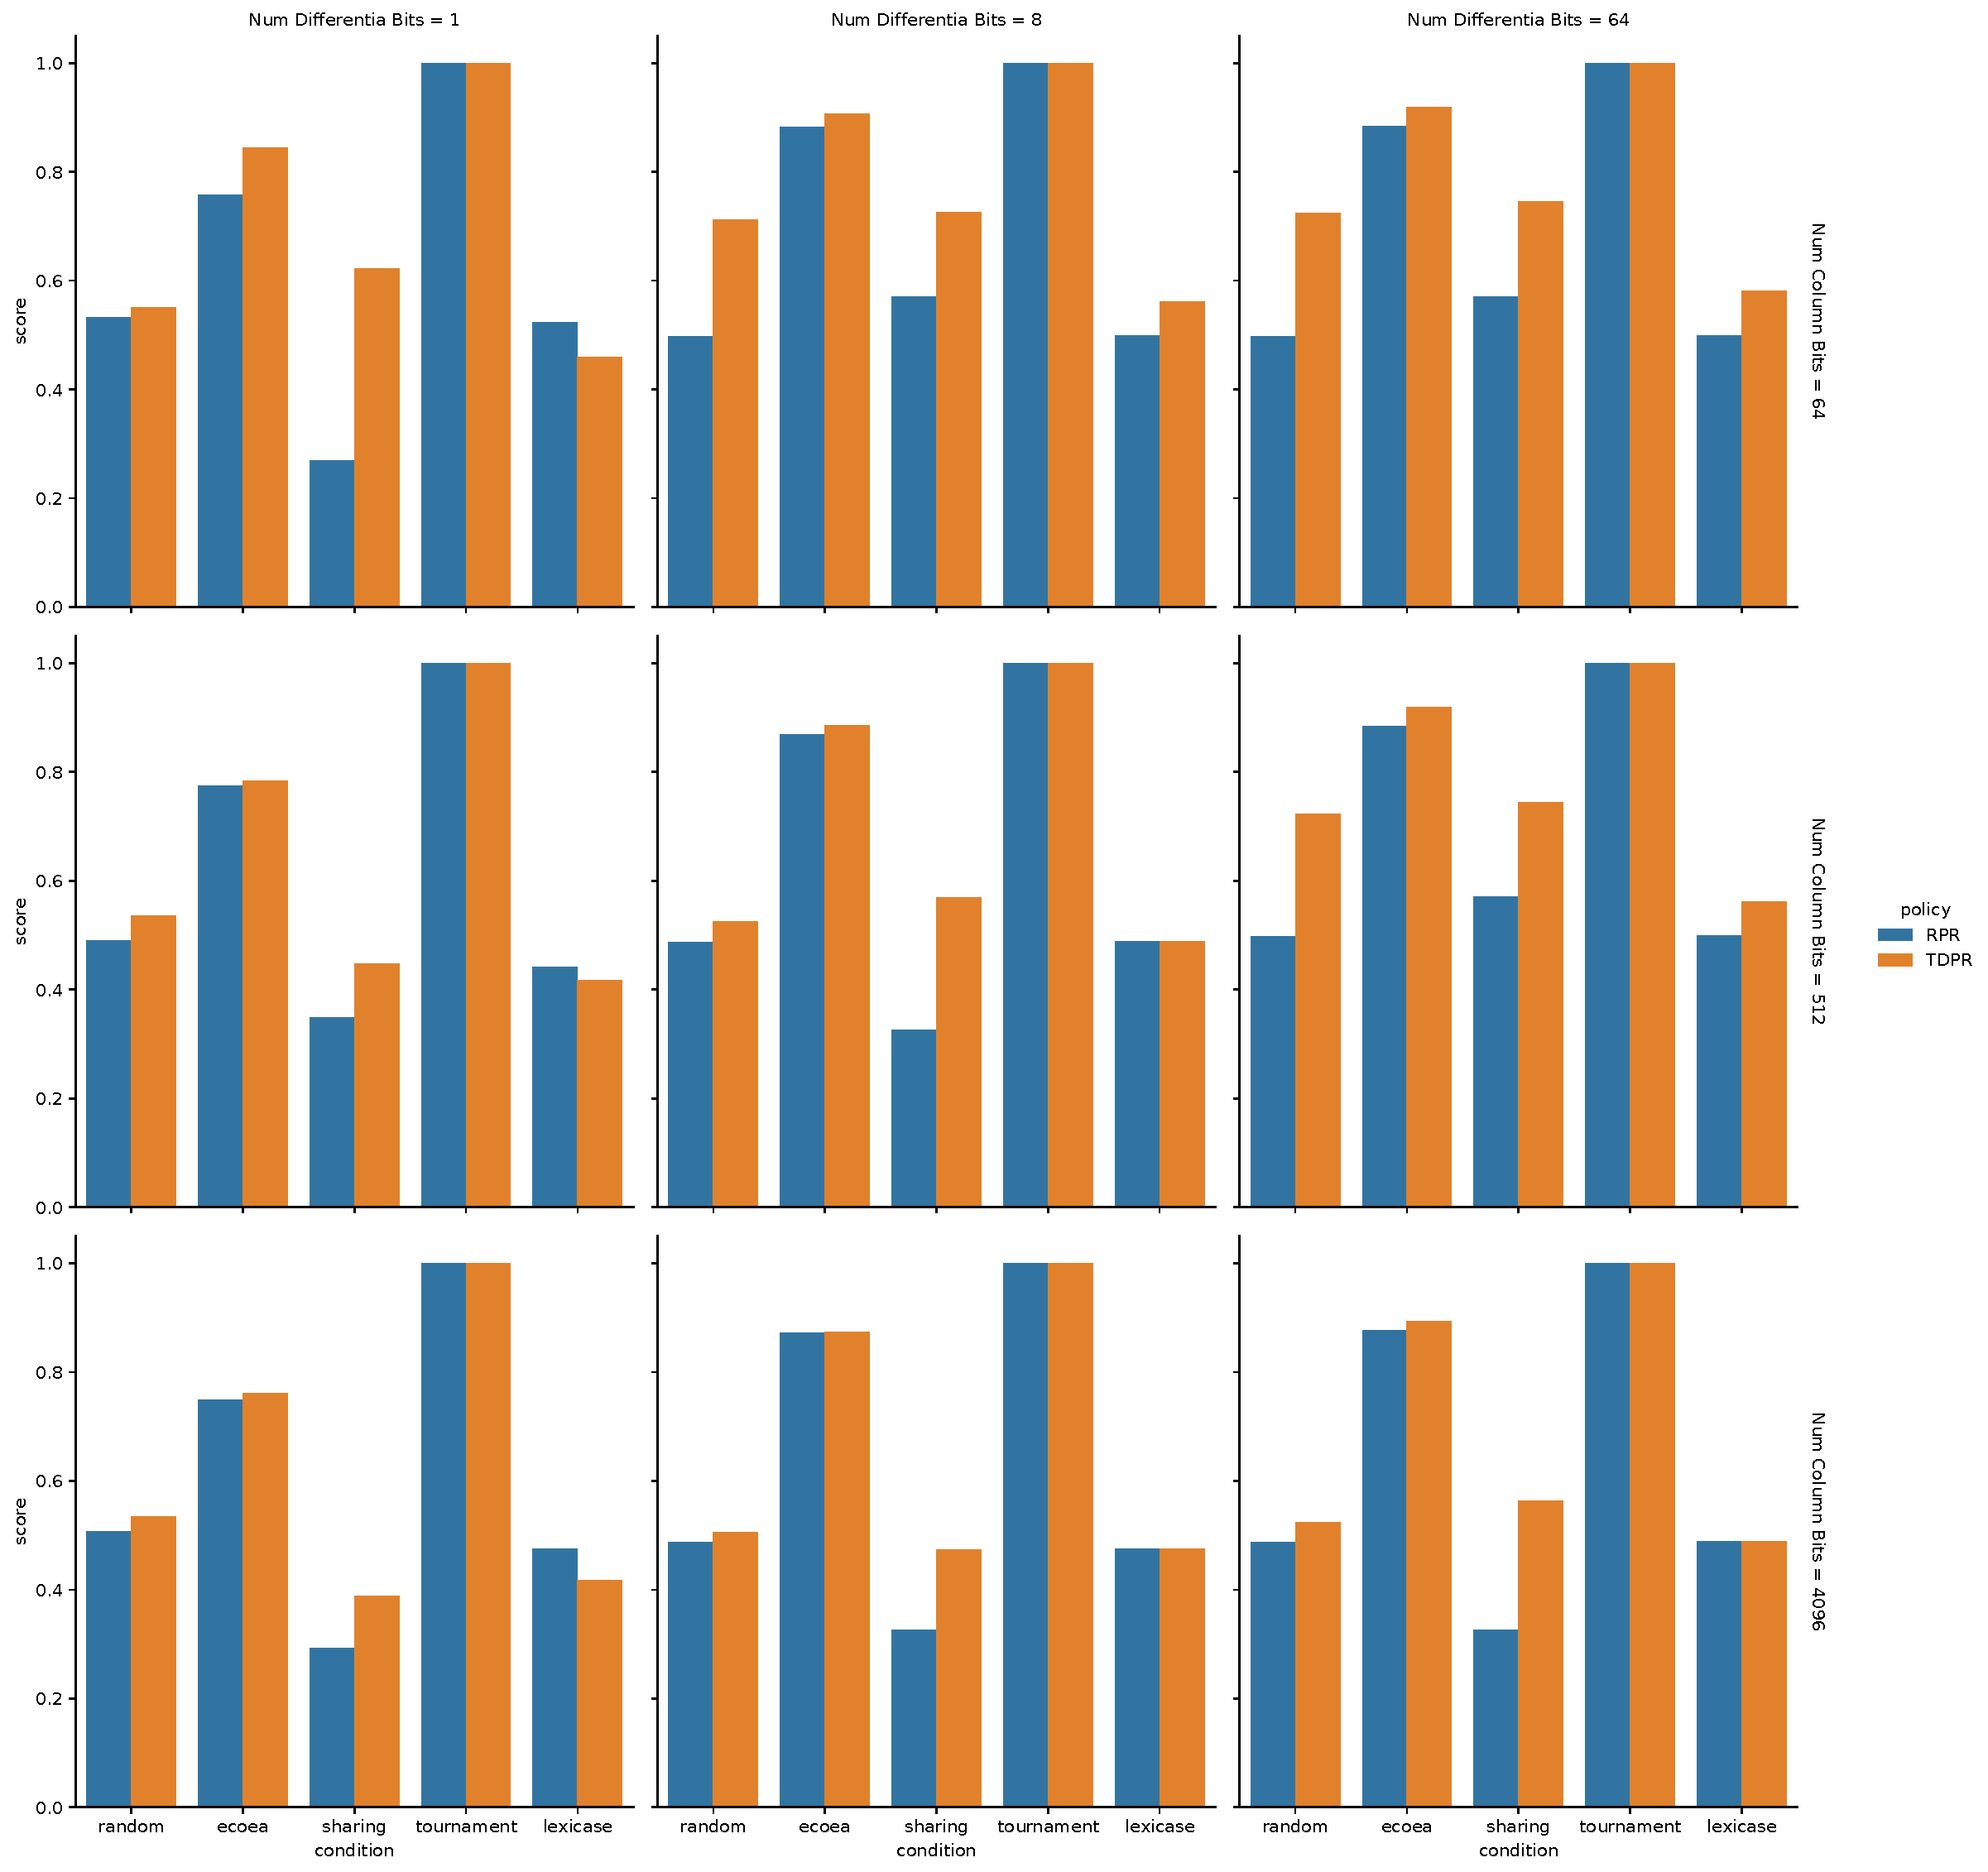
\includegraphics[width=\linewidth]{submodules/hereditary-stratigraph-concept-binder/binder/reconstruction-quality/teeplots/col=num-differentia-bits+hue=policy+kind=bar+row=num-column-bits+tree-comparison-metric=clustering-information-distance+viz=catplot+x=condition+y=score+ext=}
    \caption{
    Comparison of phylogenetic reconstruction quality between stratum retention policies.
    Reconstruction quality measured as clustering information distance between reconstructed phylogeny and ground truth phylogeny \citep{smith2020information, smith2020treedist}.
    Lower is better.
    RPR is recency-proportional resolution stratum retention policy and TDPR is tapered depth-proportional resolution stratum retention policy.
    }
    \label{fig:policy-clustering-information-distance}
\end{figure*}
